\subsection{The integral equation}
Since the fluid is ideal, we may reduce the incompressibility condition to the \textsc{Laplace} equation,
\[
\nabla^2\phi = 0, \qquad \text{in } \Omega.
\]
It may be shown with the product rule that for any harmonic functions $\phi,\psi \in \Omega$,
\[
\nabla\cdot \big( \phi\nabla\psi - \psi\nabla\phi \big) \equiv 0,
\]
which upon being integrated over $\Omega$ and applying \textsc{Gauss}' divergence theorem, yields
\[
\int_{\partial\Omega} \big( \phi\nabla\psi - \psi\nabla\phi \big) \,\dee S = 0.
\]
Since we only need the values of the potential on the contour $\partial\Omega$ to calculate the added mass, we look to \textsc{Green} functions, which are defined through the property that they satisfy some differential operator except at some point $\bzhe \in \Othal$, where $\Othal = \Omega \cup \partial\Omega$, such that
\[
\nabla^2 \green = \delta(\xvec - \bzhe), \qquad \xvec\in\Othal.
\]
In other words, the \textsc{Green} function is almost harmonic, and we expect the above integral should hold except at the pole.
The \textsc{Green} function for the \textsc{Laplace} operator is the natural logarithm,
\[
\green(\xvec) = \ln{r}, \qquad r = \absl{\xvec - \bzhe},
\]
which has a pole at $\bzhe$.
Now, by placing $\bzhe\in\partial\Omega$, we find by the \textsc{Cauchy} principal value,\footnote{\cite{lavrentev1967methoden} \textsc{Lavrentev} \& \textsc{\v{S}abat}, pp.331--332} that
\[
-\pi\phi(\bzhe) + \mathrm{pv}\int_{\partial\Omega} \phi \partial_{\nhat}\ln{r} \,\dee S = \mathrm{pv} \int_{\partial\Omega} \partial_{\nhat}\phi \ln{r} \,\dee S.
\]
An outline of calculating the principal value is found in the lecture notes from January 21\textsuperscript{st}.
We drop the principal value notation for brevity.

\subsection{The boundary element method}
To implement the integral equation numerically, we utilize the boundary element method.
In essence, we distribute a number of nodes along the boundary on which we would like to solve the integral equation, and linearily interpolate the points to approximate boundary.
If the number of nodes is $N$, then we have $\partial\Omega \sim S = \{S_n \colon n \leq N, \, n \in \mathbb{Z}^{+}\}$.
We then assume the potential is constant on each of $S_n$, equal to the potential evaluated at the midpoint, labelling this ${\phi_j}^{n} \equiv \phi_j(\zhett_n)$.
Now, since the normal derivative of the potential also must be zero on the line segments, the integrals in the integral equation may be approximated by the sum of the integrals evaluated over wach of the line segments as follows.
\begin{equation}\label{eq:deen_log_integral}
\int_{\partial\Omega} \phi \partial_{\nhat} \ln{r} \,\dee S \approx \sum_{n = 1}^{N} \phi^{n} \int_{S_n} \partial_{\nhat} \ln{r} \,\dee S
\end{equation}
\begin{equation}\label{eq:log_integral}
\int_{\partial\Omega} \ln{r} \partial_{\nhat} \phi \,\dee S \approx \sum_{n = 1}^{N} \nhat^{n} \int_{S_n} \ln{r} \,\dee S
\end{equation}
It should be quite clear that the integral equation may then be written as the matrix equation
\[
-\pi\phi^{n} + \sum_{n = 1}^{N} \phi^{n} \Thetatt_{m,n} = \sum_{n = 1}^{N} \nhat^{n} \mathtt{h}_{m,n},
\]
where we have set $\Thetatt_{m,n}$ and $\mathtt{h}_{m,n}$ to be approximations of equations \eqref{eq:deen_log_integral} and \eqref{eq:log_integral}, respectively.

\subsection{The logarithmic gradient}
It turns out the integral of the gradient of the logarithm can be determined using complex analysis.
The gradient is an operator from the real numbers into the vector space of the complex numbers, in the sense that
\[
\nabla u(\ezh) = \deex u(\ezh) + i\deez u(\ezh), \qquad \ezh = x + iz.
\]
Considering now an analytic function $\uvec = u + iv$, its complex derivative is given by $\partial_{\ezh} \uvec = \deex u + i\deex v$, which by the \textsc{Cauchy}--\textsc{Riemann} equations yields that $\partial_{\ezh} \uvec = {\nabla u}^{\ast}$.
We recall that the principal value of the complex logarithm is given by $\Log{(\ezh)} = \ln{\absl{\ezh}} + i\Arg{(\ezh)}$,\footnote{\cite{lavrentev1967methoden} \textsc{Lavrentev} \& \textsc{\v{S}abat}, p.30} so that $\partial_{\ezh} \Log{(\ezh)} = {\nabla\ln{\absl{\ezh}}}^{\ast}.$

Now, for a curve parametrized by $\lambda(s)$, the normal vector $\nhat$ may be represented by\footnote{\cite{markusevic1965theoryII} \textsc{Marku\v{s}evi\v{c}}, p.175}
\[
\nu(s) = -i \lambda^{\prime}(s) = \frac{\dee z}{\dee s} - i\frac{\dee x}{\dee s} = -i\frac{\dee \ezh}{\dee s}.
\]
The inner product may be defined such that $\uvec\cdot\nhat = \Re{(\uvec^{\ast} \nu(s))}$.
We then have that
\[
\partial_{\nhat}\ln{r} = \Re{\left( -i\frac{\dee \ezh}{\dee s} \frac{\dee}{\dee \ezh} \Log{(\ezh - \bzhe_m)} \right)}.
\]
Since the line segment is parameterized by $s$, the differential element may then be taken over $\ezh$.
By the linearity of the $\Re{(\star)}$ operator, we have that
\begin{align*}
  \int_{S_n} \partial_{\nhat} \ln{r} \,\dee S & = -\Re i \int_{{\xvec}_{n-1}}^{\xvec_n} \frac{\dee}{\dee\ezh} \Log{(\ezh - \bzhe_m)} \,\dee\ezh.\\
  & = \Arg{\left( \frac{\xvec_{n - 1} - \bzhe_m}{\xvec_n - \bzhe_m} \right)}.
\end{align*}
This is just the angle between $\xvec_n$, $\bzhe_m$, and $\xvec_{n-1}$.
\begin{Figure}
  \centering
  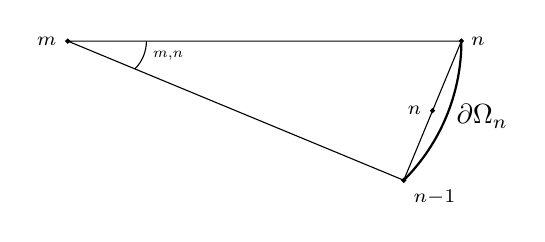
\begin{tikzpicture}
    \begin{scope}[scale = 2.5]
        \def\r{1}\def\smallr{.2}
        \def\thetai{-45}\def\thetaf{0}\def\thetam{180}
        \draw
            (
                {(1-\smallr)*\r*cos(\thetam) + \smallr*\r*cos(\thetaf)},
                {(1-\smallr)*\r*sin(\thetam) + \smallr*\r*sin(\thetaf)}
            ) arc (\thetaf:\thetai:\smallr) node[midway, right]{\scalebox{.75}{$\Thetatt_{m,n}$}};
        \draw[cap = round]
            ({\r*cos(\thetaf)}, {\r*sin(\thetaf)})--
            ({\r*cos(\thetam)}, {\r*sin(\thetam)})--
            ({\r*cos(\thetai)}, {\r*sin(\thetai)})--cycle;
        \draw[thick] ({\r*cos(\thetai)}, {\r*sin(\thetai)}) arc (\thetai:\thetaf:\r) node[midway, right]{${\partial\Omega}_{n}$};
        \draw[fill = black] ({\r*cos(\thetaf)}, {\r*sin(\thetaf)}) circle (.01) node[right]{$\xvec_n$};
        \draw[fill = black] ({\r*cos(\thetai)}, {\r*sin(\thetai)}) circle (.01) node[below right]{$\xvec_{n-1}$};
        \draw[fill = black] ({\r*cos(\thetam)}, {\r*sin(\thetam)}) circle (.01) node[left]{$\bzhe_m$};
        \draw[fill = black]
            (
                {.5*\r*cos(\thetaf) + .5*\r*cos(\thetai)},
                {.5*\r*sin(\thetaf) + .5*\r*sin(\thetai)}
            ) circle (.01) node[left]{$\bzhe_n$};
    \end{scope}
\end{tikzpicture}

  \captionsetup{type = figure}
  \caption{Visualization of $\Thetatt_{m,n}$. Here $S$ denotes the segment along $\partial\Omega$ between $\xvec_{n}$ and $\xvec_{n-1}$.}
\end{Figure}

\subsection{Approximated added mass}
Let $\delta S_{n} = \absl{\xvec_{n} - \xvec_{n - 1}}$.
\[
    \addedmass = [m_{ij}] \approx \varrho \sum_{n = 1}^{N} {\phi_{j}}^{n} {\hat{n}}_{i}{}^{n} \delta S_{n}.
\]
